% Types de problèmes (décision / optimisation)
\begin{frame}{Types de problèmes}
    \begin{block}{Problèmes de décision}
        Problèmes auxquels on peut répondre par oui ou non.
        \begin{itemize}
            \item \textbf{Problème du plus court chemin} : existe-t-il un chemin de coût $\leq k$ entre deux n\oe{}uds $s$ et $t$ dans un graphe pondéré ?
            \item \textbf{Problème du cycle hamiltonien} : existe-t-il un cycle passant par tous les n\oe{}uds d'un graphe exactement une fois ?
        \end{itemize}
    \end{block}

    \begin{block}{Problèmes d'optimisation}
        Problèmes dans lesquels on cherche la solution de coût minimal (ou maximal).
        \begin{itemize}
            \item \textbf{Problème du plus court chemin} : quel est le chemin le plus court entre les n\oe{}uds $s$ et $t$ dans un graphe pondéré ?
            \item \textbf{Problème du voyageur de commerce} : trouver un cycle hamiltonien de poids minimum.
        \end{itemize}
    \end{block}
\end{frame}

% Méthode
\begin{frame}{Formaliser un problème}
    Pour formaliser un problème, on donne ses entrées (instances), et la question à laquelle on veut répondre.
    \bigskip
    \begin{exampleblock}{Exemple}
        Formaliser le problème du plus court chemin entre deux n\oe{}uds $s$ et $t$ dans un graphe pondéré sous forme de problème de décision.
        \medskip

        \textbf{Entrées} :
        \begin{itemize}
            \item Un graphe $G=(V,E,w)$ pondéré
            \item Des n\oe{}uds $s,t\in V^2$
            \item Un nombre $k\in \mathbb{N}$
        \end{itemize}

        \textbf{Question} : existe-t-il un chemin $C\subseteq E$ de $s$ à $t$ tel que :
        \[
            \sum_{c\in C} w(c) \leq k
        \]
    \end{exampleblock}
\end{frame}

\begin{frame}{Types de problèmes}
    \begin{alertblock}{Attention !}
        Dans tout ce qui suit, on s'intéresse uniquement à des \textbf{problèmes de décision}.
    \end{alertblock}
\end{frame}

% Classes (définitions)
\begin{frame}{Classes P et NP}
    Dans le cas des \textbf{problèmes de décision} uniquement, on peut définir les classes de complexité \textbf{P} et \textbf{NP}.

    \begin{block}{Classe P}
        Un problème est dans la classe P s'il peut être résolu par un algorithme en complexité polynomiale.
    \end{block}

    \begin{block}{Classe NP}
        Un problème est dans la classe NP si ses solutions peuvent être vérifiées par un algorithme en temps polynomial.
        \medskip

        Pour montrer qu'un problème est dans NP, il suffit de donner un algorithme de vérification et de montrer qu'il est polynomial.
    \end{block}

    On a naturellement $P \subseteq NP$.
\end{frame}

% Réduction polynomiale
\begin{frame}{Réductions de problèmes}
    \begin{block}{Instance et instance positive}
        Soit un problème $\mathcal{P}$. On note $\mathcal{D}$ les instances (ou entrées) possibles pour $\mathcal{P}$ (e.g l'ensemble des graphes).
        \smallskip

        On a $\mathcal{D} = \mathcal{D}^+ \sqcup \mathcal{D}^-$ (union disjointe) où :
        \begin{itemize}
            \item $\mathcal{D}^+$ est l'ensemble des entrées pour lesquelles la réponse au problème est oui (instances positives) ;
            \item $\mathcal{D}^-$ est l'ensemble des entrées pour lesquelles la réponse au problème est non (instances négatives).
        \end{itemize}
    \end{block}

    \begin{block}{Réduction}
        On dit qu'un problème $\mathcal{P}_1$ se réduit à un autre problème $\mathcal{P}_2$ s'il existe une fonction $tr$ qui transforme une entrée de $\mathcal{P}_1$ en entrée de $\mathcal{P}_2$ en temps polynomial, telle que $e \in \mathcal{D}_1^+$ ssi $tr(e) \in \mathcal{D}_2^+$.
    \end{block}
\end{frame}

% Schéma réduction
\begin{frame}{Réduction de problèmes}
    \begin{center}
        \includegraphics[width=0.6\textwidth]{images/reduction}
    \end{center}
\end{frame}

% Définitions
\begin{frame}{Problèmes NP-difficiles et NP-complets}
    \begin{block}{Problème NP-difficile}
        Un problème $\mathcal{P}_1$ est dit NP-difficile si tout problème de la classe NP peut s'y réduire.
        \medskip

        En pratique pour montrer que $\mathcal{P}_1$ est NP-complet, on trouve une réduction d'un problème NP-complet $\mathcal{P}_c$ à $\mathcal{P}_1$.
    \end{block}

    \begin{center}
        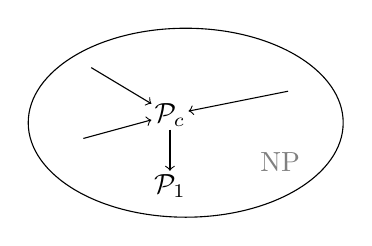
\begin{tikzpicture}
            \draw (0,0) ellipse [x radius=2cm, y radius=1.2cm];
            \node[text=gray] at (1.2,-.5) {NP};

            \node[inner sep=1pt] (Pc) at (-.2, .1) {$\mathcal{P}_c$};
            \node[inner sep=1pt] (P1) at (-.2, -.8) {$\mathcal{P}_1$};

            \draw[->] (-1.3, -.2) -- (Pc);
            \draw[->] (-1.2, .7) -- (Pc);
            \draw[->] (1.3, .4) -- (Pc);
            \draw[->] (Pc) -- (P1);
        \end{tikzpicture}
    \end{center}

    \begin{block}{Problème NP-complet}
        Un problème est dit NP-complet s'il est \textbf{dans la classe NP} et qu'il est \textbf{NP-difficile}.
    \end{block}
\end{frame}

% Exemple de réduction
\begin{frame}{Exemple de réduction}
    On se propose de réduire le problème \textsc{Chemin Hamiltonien} (NP-difficile) vers \textsc{Plus Long Chemin} pour montrer que \textsc{Plus Long Chemin} est NP-difficile.

    \begin{exampleblock}{Chemin Hamiltonien}
        \textbf{Entrées} : un graphe non orienté connexe $G=(V,E)$
        \smallskip

        \textbf{Question} : existe-t-il un chemin simple (sans cycle) qui visite tous les sommets de $G$ ?
    \end{exampleblock}

    \begin{exampleblock}{Plus long chemin}
        \textbf{Entrées} : un graphe non orienté pondéré connexe $G=(V,E,w)$ et un entier $k\in\mathbb{N}$
        \smallskip

        \textbf{Question} : existe-t-il un chemin simple $C$ dans $G$ tel que la somme des poids des arêtes de $C$ soit au moins $k$ ?
    \end{exampleblock}
\end{frame}

% Rédaction de la réduction
\begin{frame}{Exemple de réduction}
    On propose $tr(\langle G=(V,E) \rangle) = \langle G'=(V,E,w), k\rangle$ où $w(e)=1$ $\forall e \in E$ et $k=|V| - 1$.
    \medskip

    Il faut montrer que $\mathcal{I}_{Ham} \in \mathcal{D}_{Ham}^+ \iff tr(\mathcal{I}_{Ham}) \in \mathcal{D}_{PLC}^+$
    \medskip

    \boxed{\Rightarrow} Soit $\mathcal{I}_{Ham} = \langle G=(V,E) \rangle$ une instance positive du problème du chemin hamiltonien. Vu $\mathcal{I}_{Ham}\in\mathcal{D}_{Ham}^+$, il existe un chemin hamiltonien dans $G$, qui par définition contient $|V|-1$ arêtes. Dans $\mathcal{I}_{PLC}=tr(\mathcal{I}_{Ham})$, le chemin est de poids $|V|-1 = k$.\\
    Donc $\mathcal{I}_{PLC} \in \mathcal{D}_{PLC}^+$.
    \medskip

    \boxed{\Leftarrow} Réciproquement, si $\mathcal{I}_{PLC}$ est une instance positive du problème plus long chemin, il existe un chemin simple de poids au moins $k=|V|-1$. Comme chaque arête est de poids 1, il doit visiter au moins $k+1=|V|$ sommets. Le chemin étant simple (pas de répétition de sommets), on a un chemin hamiltonien.\\
    Donc $\mathcal{I}_{Ham} \in \mathcal{D}_{Ham}^+$.
    \medskip

    On a réduit Ham (NP-difficile) à PLC donc PLC est NP-difficile.
\end{frame}

% Méthode pour montrer la NP-complétude
\begin{frame}{Méthode pour montrer la NP-complétude}
    Pour montrer qu'un problème est \textbf{NP-complet} :
    \bigskip

    \begin{enumerate}
        \item On montre que le problème est \textbf{dans NP} en exhibant un algorithme de vérification de complexité polynomiale ;
        \item On montre que le problème est \textbf{NP-difficile} en réduisant un autre problème NP-difficile à lui ;
        \item On conclut en disant que NP \& NP-difficile $\iff$ NP-complet
    \end{enumerate}
\end{frame}

% Problèmes classiques (cours + TD)
\begin{frame}{Problèmes NP-complets classiques}
    \begin{exampleblock}{SAT}
        \textbf{Entrée} : une formule logique sous FNC e.g $(x_1 \lor x2) \land (\lnot x_1)$
        \smallskip

        \textbf{Question} : la formule est-elle satisfiable ?
    \end{exampleblock}

    \begin{exampleblock}{Stable}
        \textbf{Entrées} : un graphe non-orienté connexe $G=(V,E)$ ; $k\in \mathbb{N}$
        \smallskip

        \textbf{Question} : existe-t-il un stable $S$ de $G$, càd un ensemble de sommets qui ne sont pas reliés entre eux par une arête, tel que $|S| \geq k$ ?
    \end{exampleblock}

    \begin{exampleblock}{Vertex-Cover}
        \textbf{Entrées} : un graphe non-orienté connexe $G=(V,E)$ ; $k\in \mathbb{N}$
        \smallskip

        \textbf{Question} : existe-t-il un ensemble $V' \subseteq V$ de taille $|V'| \leq k$ tel que toute arête $(u,v) \in E$ a au moins une de ses extrémités dans $V'$ ($u \in V'$ ou $v \in V'$) ?
    \end{exampleblock}
\end{frame}

% Problèmes classiques (cours + TD)
\begin{frame}{Problèmes NP-complets classiques}
    \begin{exampleblock}{Set-Cover}
        \textbf{Entrées} : un ensemble d'éléments $U$ ; une famille $S \subset \mathcal{P}(U)$ de sous ensembles de $U$; un nombre $k\in \mathbb{N}$
        \smallskip

        \textbf{Question} : existe-il une sous-famille $S' \subseteq S$ telle que :
        \begin{itemize}
            \item $S'$ est une couverture de $U$, càd $U = \cup_{S_i \in S'}S_i$
            \item $card(S') \leq k$
        \end{itemize}
    \end{exampleblock}

    \begin{exampleblock}{Clique}
        \textbf{Entrées} : un graphe $G=(V,E)$ ; $k\in \mathbb{N}$
        \smallskip

        \textbf{Question} : existe-il un ensemble $S \subseteq V$ tel que :
        \begin{itemize}
            \item $\forall u,v\in S^2$, $(u,v) \in E$ (le sous graphe induit est complet)
            \item $|S| \geq k$
        \end{itemize}
    \end{exampleblock}
\end{frame}

% Points importants pour l'examen
\begin{frame}{Conclusion de la section 2}
    Choses à savoir faire pour l'examen :
    \begin{itemize}
        \item Formaliser/modéliser un problème (donner entrées et question)
        \item Donner la nature d'un problème (décision ou optimisation)
        \item Connaître les problèmes classiques et leur classe
        \item Montrer qu'un problème est NP-complet (dans NP + NP-difficile)
    \end{itemize}
    \medskip

    Comment s'entraîner :
    \begin{itemize}
        \item Refaire le TD 1 (tous les exercices), le TD 2 (toutes les questions sauf la 1.3 et la 2.2), et le TD 3 (exercice 1, questions 1 à 4).
    \end{itemize}
\end{frame}
